% ---------------------------------------------------------------
% 3.2  V-MARCH Overview
% ---------------------------------------------------------------
\subsection{\ours Overview}
\label{sec:overview}

\begin{figure*}[t]
    \centering
    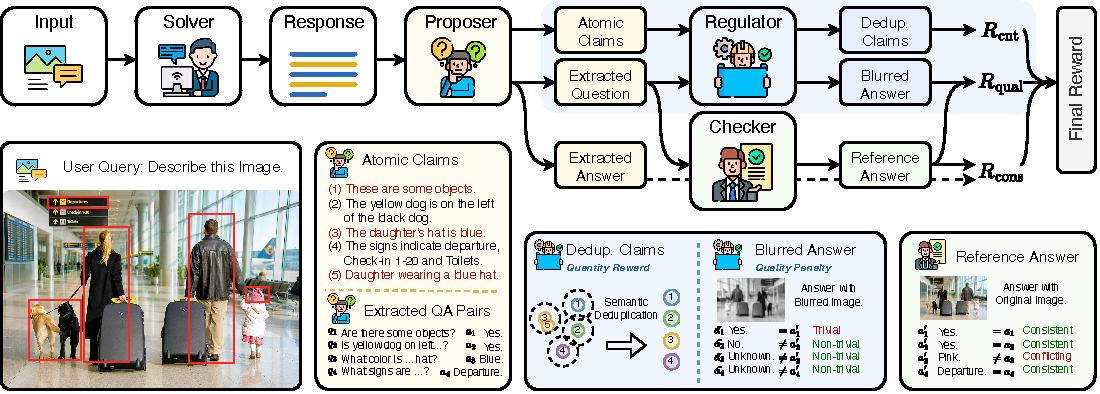
\includegraphics[width=\textwidth]{figures/v-march-pipeline-final.pdf}
    \caption{Overview of the \ours pipeline.
    Given a \textbf{Solver}-generated response, the \textbf{Proposer} decomposes it into atomic factual claims and converts each into a visual question-answer pair.
    The \textbf{Regulator} performs Visual Claim Regulation (VCR) by deduplicating semantically redundant claims, rewarding claim quantity, and penalizing image-agnostic claims that can be answered without genuine visual perception.
    The \textbf{Checker} re-answers each question using the original image, and verifies consistency with the Solver's answers.
    The final self-verifying reward aggregates the Checker's consistency signal and the Regulator's quantity and quality signals.
    }
    \label{fig:pipeline}
\end{figure*}

\ours adapts the Proposer--Checker paradigm~\cite{wang2026visionzero,li2026march} to the visual domain and extends it with a dedicated \textbf{Regulator} agent.
The Regulator governs the quantity and quality of the claim set, addressing unreliable rewards to visual self-verification.
As illustrated in Figure~\ref{fig:pipeline}, \ours orchestrates four agents in a sequential pipeline:

\begin{itemize}[leftmargin=1em,itemsep=2pt]
\item \textbf{Solver.} Generates a response $\vy$ conditioned on the
    image--instruction pair $(\mI, \vq)$.
    Only the Solver is updated by GRPO training.
\item \textbf{Proposer.} Decomposes $\vy$ into a set of
    atomic factual claims $\mathcal{C} = \{\vc_1, \ldots, \vc_m\}$ and
    converts each claim into a visual question-answer pair, yielding the
    raw claim set $\mathcal{Q} = \{(\vv_i, \va_i)\}_{i=1}^{m}$.
\item \textbf{Regulator.} Audits $\mathcal{Q}$ by
    (i)~removing semantically redundant claims to prevent reward inflation
    via repetition, yielding the filtered set
    $\mathcal{Q}^{\ast} = \{(\vv_i, \va_i)\}_{i=1}^{n}$, $n \leq m$;
    (ii)~rewarding sufficient claim coverage via a claim-count signal
    $r^{\text{cnt}}$; and (iii)~penalizing image-agnostic claims that
    can be resolved without genuine visual perception via a quality signal
    $r^{\text{qual}}$. 
    We refer to the claim-level quantity and quality control as \textbf{Visual Claim Regulation} (VCR), which is described in detail in Section~\ref{sec:regulator}.
\item \textbf{Checker.} Receives the original image $I$ and questions $\{\vv_i\}$ from $\mathcal{Q}^{\ast}$, with no access to $\vy$.
    It generates image-grounded reference answers $\{\va_i'\}$ and verifies
    consistency with the claim-implied answers $\{\va_i\}$ via majority
    voting, producing a consistency reward $r^{\text{cons}}$.
\end{itemize}

The final self-verifying reward aggregates signals from the Regulator and
the Checker:
\begin{equation}
    r^{\text{SV}}(\mI, \vq, \vy)
    = \underbrace{r^{\text{cons}}}_{\text{Checker}}
    + \underbrace{r^{\text{cnt}} + r^{\text{qual}}}_{\text{Regulator}}.
    \label{eq:reward_total}
\end{equation}
This reward is used directly as the GRPO training signal for the Solver,
requiring no human annotation or external supervision.


% \begin{equation}
%     r^{\text{SV}}(I, q, y)
%     = \underbrace{r^{\text{cons}}}_{\text{Checker}}
%     + \underbrace{r^{\text{cnt}} + r^{\text{qual}}}_{\text{Regulator}}.
%     \label{eq:reward_total}
% \end{equation}
% This \emph{information asymmetry}---the Checker observes the image but not the generated description---breaks the self-confirmation bias inherent in single-model verification.


% ---------------------------------------------------------------
% 3.3  Proposer: Claim Extraction
% ---------------------------------------------------------------
\subsection{Proposer: Claim Extraction}
\label{sec:proposer}

Given $\vy$, the Proposer extracts a set of atomic factual
claims:
\begin{equation}
    \mathcal{C} = \{\vc_1, \ldots, \vc_m\} = \text{Extract}(\vy),
\end{equation}
where each $c_i$ is a short, self-contained statement about a single visual
fact (e.g., object existence, color, quantity, or spatial relation).
Each claim is then converted into a visual question-answer pair:
\begin{equation}
    (\vv_i,\, \va_i) = \text{QA}(\vc_i),
    \qquad i = 1, \ldots, m,
\end{equation}
where $\va_i$ is the answer implied by the claim.
The resulting raw claim set $\mathcal{Q} = \{(\vv_i, \va_i)\}_{i=1}^{m}$
is passed to the Regulator for quality control.

\smallskip
\noindent\textit{Example.}
For the query ``Describe this image'' applied to an airport scene, the Solver might generate a response $\vy$. 
The Proposer then extracts atomic claims and converts each to a QA pair, for instance:
\textit{``The yellow dog is on the left of the black dog''} $\to$ (Q: \textit{Is the yellow dog on the left of the black dog?}, A: \textit{Yes});
\textit{``The daughter's hat is blue''} $\to$ (Q: \textit{What color is the daughter's hat?}, A: \textit{Blue}).
% \textit{``The signs indicate Departure, Check-in 1--20, and Toilets''} $\to$ (Q: \textit{What signs are indicated?}, A: \textit{Departure, Check-in 1--20, Toilets}).
% These raw QA pairs are forwarded to the Regulator.


% ---------------------------------------------------------------
% 3.4  Regulator: Visual Claim Regulation
% ---------------------------------------------------------------
\subsection{Regulator: Visual Claim Regulation}
\label{sec:regulator}

The Regulator addresses degenerate behaviors that undermine the reliability of visual self-verification if left unchecked:
(1)~a model can repeat near-identical claims to inflate $r^{\text{cons}}$;
(2)~it can produce easily verified claims to obtain a stable reward while remaining under-informative;
(3)~it can generate image-agnostic claims (e.g., \textit{``the image contains objects''}) whose answers follow from language priors rather than genuine visual perception.
The Regulator counteracts these through semantic deduplication and complementary reward signals.

\paragraph{Semantic Deduplication.}
% To address failure mode~(1), the Regulator 
Removing semantically overlapping
claims from $\mathcal{Q}$ using cosine similarity over sentence embeddings
$\phi(\cdot)$:
\begin{equation}
    \text{Sim}(\vc_i, \vc_j)
    = \frac{\phi(\vc_i)^{\top} \phi(\vc_j)}
           {\|\phi(\vc_i)\| \cdot \|\phi(\vc_j)\|}.
\end{equation}
Pairs exceeding a type-aware similarity threshold are merged, yielding the
deduplicated claim set $\mathcal{Q}^{\ast} = \{(\vv_i, \va_i)\}_{i=1}^{n}, n \leq m$.
% , which is forwarded to the Checker for verification.

\smallskip
\noindent\textit{Example.}
Continuing the airport-scene example, the claim \textit{``Daughter wearing a blue hat''} is identified as a near-duplicate of \textit{``The daughter's hat is blue''} and is removed, reducing the claim set from $m=5$ to $n=4$ deduplicated claims.

\paragraph{Quantity Reward.}
% To address failure mode~(2), the Regulator 
The Regulator then adds a claim-count reward
proportional to the number of deduplicated claims $n$, capped at a target
$n_{\text{target}}$:
\begin{equation}
    r^{\text{cnt}}
    = \lambda_{\text{cnt}}
      \cdot \min (\frac{n}{n_{\text{target}}},1),
\end{equation}
with $\lambda_{\text{cnt}} = 0.5$ so that factual consistency remains
the dominant signal.
Because $n$ counts only deduplicated claims, failure modes~(1) and~(2)
are addressed jointly: repetition neither inflates $n$ nor contributes
to $r^{\text{cnt}}$.

\paragraph{Quality Penalty.}
To address failure mode~(3), we construct a degraded image
$\tilde{\mI}$ by applying a heavy Gaussian blur, grayscale conversion, and
horizontal flipping to $I$.
It then re-answers each question $v_i$ in $\mathcal{Q}^{\ast}$ with the
degraded image:
\begin{equation}
    \tilde{\va}_i = \text{Ans}(\tilde{\mI},\, \vv_i).
\end{equation}
If $\tilde{\va}_i$ remains consistent with the original reference answer
$\va_i'$, the claim is marked trivial, i.e., answerable without meaningful visual content.
% \begin{equation}
%     t_i = \bm{1}\!\left[
%         \gF(\tilde{a}_i,\, a_i') = 1
%     \right].
% \end{equation}
The Regulator penalizes trivial proportions:
\begin{equation}
    r^{\text{qual}} = -\lambda_{\text{qual}} \sum_{i=1}^{n} \bm{1}[
       \gF(\tilde{\va}_i,\, \va_i') = 1],
\end{equation}
pushing the Solver toward responses that require genuine image grounding.

\smallskip
\noindent\textit{Example.}
In the airport-scene example, the claim \textit{``There are some objects in the image''} yields the blurred-image answer \textit{``Yes,''} which is consistent with the reference answer; accordingly, $\bm{1} [\gF(\tilde{\va}_i,  \va_i') = 1]$=1 and this claim incurs a quality penalty.
By contrast, \textit{``The yellow dog is on the left of the black dog''} cannot be reliably answered from the degraded image, no penalty is applied.


% ---------------------------------------------------------------
% 3.5  Checker: Image-Grounded Verification
% ---------------------------------------------------------------
\subsection{Checker: Image-Grounded Verification}
\label{sec:checker}

The Checker receives the filtered claim set $\mathcal{Q}^{\ast}$ output by
the Regulator and the original image $I$, with no access to
$\vy$.
For each question $v_i \in \mathcal{Q}^{\ast}$, it generates an
image-grounded reference answer:
\begin{equation}
    \va_i' = \text{Ans}(\mI, \vv_i),
\end{equation}
and verifies consistency with the claim-implied answer via majority voting
over $K$ independent runs:
\begin{equation}
    \vz_i = \bm{1}[
        \sum_{k=1}^{K} \vz_i^{(k)} > \frac{K}{2}],
    \ \ 
    \vz_i^{(k)} = \gF(\va_i,\, \va_i').
\end{equation}
The resulting consistency reward is
\begin{equation}
    r^{\text{cons}} = \frac{1}{n} \sum_{i=1}^{n} z_i,
\end{equation}
measuring the fraction of claims in $\mathcal{Q}^{\ast}$ that are supported
by image-grounded evidence.
% This \emph{information asymmetry}---the Checker observes the image but not
% the Solver's response---prevents the verifier from inheriting the same
% hallucination tendencies as the generator, thereby producing a more reliable
% consistency signal than single-model self-verification.

\paragraph{Final Reward.}
Combining the Checker and Regulator signals, the total reward used for
GRPO training is~\eqref{eq:reward_total}.
% \begin{equation}
%     r^{\text{SV}}(I, q, y)
%     = r^{\text{cons}} + r^{\text{cnt}} + r^{\text{qual}}.
% \end{equation}
The three terms are complementary: $r^{\text{cons}}$ enforces factual
grounding; $r^{\text{cnt}}$ promotes visual coverage; and
$r^{\text{qual}}$ filters out image-agnostic claims.
Together, the multi-agent pipeline provides a reliable, annotation-free
reward signal for scalable hallucination mitigation in VLMs.
